% (The MIT License)
%
% Copyright (c) 2023-2024 Yegor Bugayenko
%
% Permission is hereby granted, free of charge, to any person obtaining a copy
% of this software and associated documentation files (the 'Software'), to deal
% in the Software without restriction, including without limitation the rights
% to use, copy, modify, merge, publish, distribute, sublicense, and/or sell
% copies of the Software, and to permit persons to whom the Software is
% furnished to do so, subject to the following conditions:
%
% The above copyright notice and this permission notice shall be included in all
% copies or substantial portions of the Software.
%
% THE SOFTWARE IS PROVIDED 'AS IS', WITHOUT WARRANTY OF ANY KIND, EXPRESS OR
% IMPLIED, INCLUDING BUT NOT LIMITED TO THE WARRANTIES OF MERCHANTABILITY,
% FITNESS FOR A PARTICULAR PURPOSE AND NONINFRINGEMENT. IN NO EVENT SHALL THE
% AUTHORS OR COPYRIGHT HOLDERS BE LIABLE FOR ANY CLAIM, DAMAGES OR OTHER
% LIABILITY, WHETHER IN AN ACTION OF CONTRACT, TORT OR OTHERWISE, ARISING FROM,
% OUT OF OR IN CONNECTION WITH THE SOFTWARE OR THE USE OR OTHER DEALINGS IN THE
% SOFTWARE.

\documentclass{article}
\usepackage{../sqm}
\usepackage{amsmath}
\usepackage{relsize}
\newcommand*\thetitle{Dead Code}
\begin{document}

\plush{\sqmTitlePage{12}{zN0gX9m6a2k}}

\pptBanner{Motivating Example}
\begin{multicols}{2}
Before (\textcolor{red}{wrong}):\par
{\small\begin{ffcode}
class Book
  private int id;
  public Book(int it)
    this.id = i;
  public int getId()
    return this.id;

  private int setId(int i)
    this.id = i;
\end{ffcode}
}
\par\columnbreak\par
After (\textcolor{green}{better}):\par
{\small\begin{ffcode}
class Book
  private final int id;
  public Book(int it)
    this.id = i;
  public int getId()
    return this.id;
\end{ffcode}
}
\end{multicols}
\plush{}

\qte
  [Mika M\"{a}ntyl\"{a}]
  {mika-mantyla.jpg}
  {Dead code is code that has been used in the past, but is currently never executed. Dead code \ul{hinders} code \ul{comprehension} and makes the current program structure \ul{less obvious}.}
  {mantyla2003}

\pptBanner{Dead Code Elimination (Compiler Optimization)}
\begin{multicols}{2}
Dead code is here:\par
{\small\begin{ffcode}
void main(int x) {
  int a = 42;
  if (x > 0) {
    a = 256;
  }
  a = 7;
  print(a);
}
\end{ffcode}
}
\par\columnbreak\par
``Dead code refers to computations whose \ul{results are never used}. Code that is dead can be eliminated without affecting the behavior of the program.''\par
{\scriptsize Source: \textit{Compiler Techniques for Code Compaction}, Saumya K. Debray, William Evans, Robert Muth, Bjorn De Sutter, ACM Transactions on Programming languages and Systems (TOPLAS), 22(2), 2000 \par}
\end{multicols}
\plush{}

\qte
  [Simone Romano]
  {simone-romano.jpg}
  {Although there is some consensus on the fact that dead code is a common phenomenon, it could be \ul{harmful}, and it seems to matter to software professionals; surprisingly, dead code has received very little empirical attention from the software engineering research community.}
  {romano2018}

\plush{\pptBanner{Unreachable/Dead Methods in Java}\pptPic{.9}{unreachable.png}\par{\scriptsize Source: \textit{A Graph-based Approach to Detect Unreachable Methods in Java Software}, Simone Romano, Giuseppe Scanniello, Carlo Sartiani, Michele Risi, Proceedings of the 31st Annual ACM Symposium on Applied Computing, 2016\par}}

\qte
  [Sebastian Eder]
  {sebastian-eder.jpg}
  {We conducted the study on the level of methods in the sense of object oriented programming. The systems contains 25,390 methods. We found that \ul{25\% of all methods} were never used during the complete period.}
  {eder2012}

\plush{
\pptBanner{Volatility Metric}
\begin{multicols}{2}
\scalebox{.7}{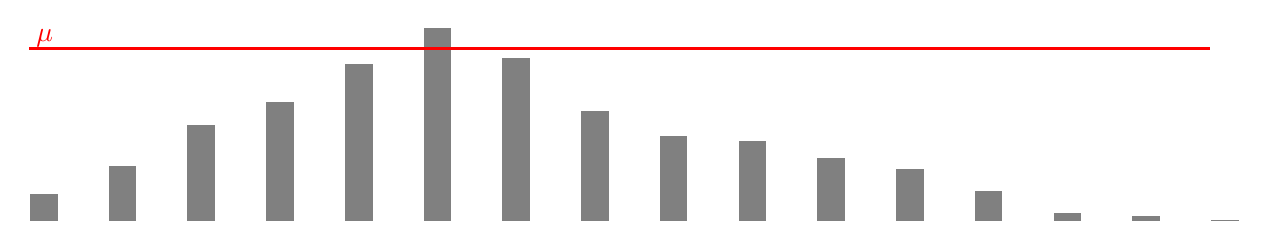
\begin{tikzpicture}[every node/.style={rectangle, minimum width=1em, fill=gray, anchor=south west, font={\color{white}}, inner sep=0pt}]
\node[minimum height=1em] at (0,0) {};
\node[minimum height=2em] at (1,0) {};
\node[minimum height=3.5em] at (2,0) {};
\node[minimum height=4.3em] at (3,0) {};
\node[minimum height=5.7em] at (4,0) {};
\node[minimum height=7em] at (5,0) {};
\node[minimum height=5.9em] at (6,0) {};
\node[minimum height=4em] at (7,0) {};
\node[minimum height=3.1em] at (8,0) {};
\node[minimum height=2.9em] at (9,0) {};
\node[minimum height=2.3em] at (10,0) {};
\node[minimum height=1.9em] at (11,0) {};
\node[minimum height=1.1em] at (12,0) {};
\node[minimum height=0.3em] at (13,0) {};
\node[minimum height=0.2em] at (14,0) {};
\node[minimum height=0.05em] at (15,0) {};
\draw[color=red, very thick] (0,2.2) node[fill=none] {\(\mu\)} -- (15,2.2);
\end{tikzpicture}}
\par
``The variance \(Var(g)\) is the \textbf{Volatility} of the source code.
The smaller the Volatility the more \textit{cohesive} is the repository
and the smaller the amount of the abandoned code inside it.''
\par\columnbreak\par
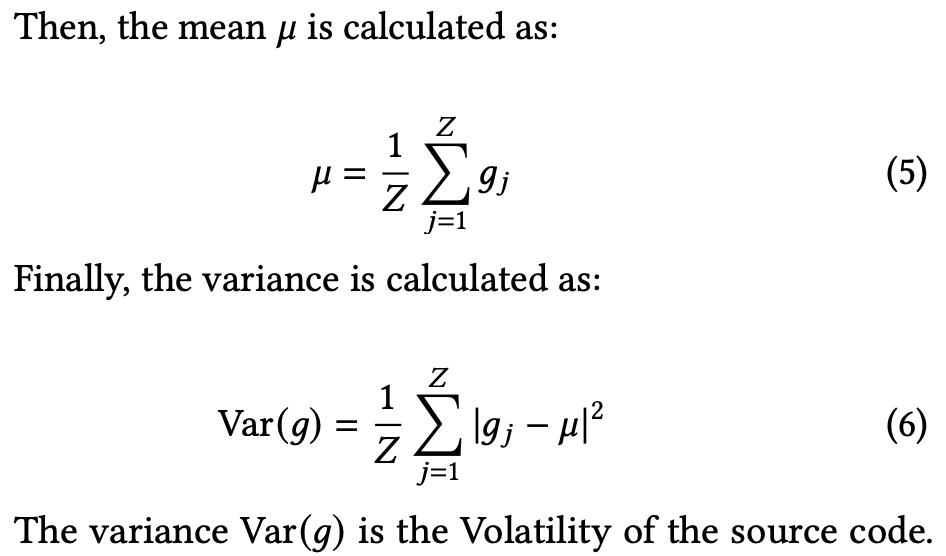
\includegraphics[width=.95\columnwidth]{formula.png}
\end{multicols}}

\plush{\pptBanner{Volatility vs. Number of Files in a Repo}\pptPic{.7}{graph.png}}

\pitch{\pptBanner{Monolithic Repositories}
{\small\begin{description}
\item[Centralization]
  The codebase is contained in a single repo encompassing multiple projects.
\item[Visibility]
  Code is viewable and searchable by all engineers in the organization.
\item[Synchronization:]
  The development process is trunk-based; engineers commit to the head of the repo.
\item[Completeness]
  Any project in the repo can be built only from dependencies also checked into the repo.
  Dependencies are unversioned; projects must use whatever version of their dependency is at the repo head.
\item[Standardization]
  A shared set of tooling governs how engineers interact with the code, including building, testing, browsing, and reviewing code.
\end{description}}\par
{\scriptsize Source: \textit{Advantages and Disadvantages of a Monolithic Repository: A case study at Google}, Ciera Jaspan et al., ICSE, 2018\par}}

\qte
  [Ciera Jaspan]
  {ciera-jaspan.jpg}
  {Our survey results show that engineers at Google strongly prefer our monolithic repo, and that \ul{visibility} of the codebase and simple \ul{dependency management} were the primary factors for this preference.}
  {jaspan2018}

\qte
  [Rachel Potvin]
  {rachel-potvin.jpg}
  {The Google codebase includes approximately \ul{one billion files} and has a history of approximately 35 million commits spanning Google's entire 18-year existence. The repository contains \ul{86TBa} of data, including approximately \ul{two billion lines of code} in nine million unique source files.}
  {potvin2016}

\qte
  [Durham Goode]
  {durham-goode.jpg}
  {Facebook's main source repository is enormous---many times larger than even the Linux kernel, which checked in at \ul{17 million lines of code} and \ul{44,000 files} in 2013.}
  {goode2014}

\qte
  [Tomas Votruba]
  {tomas-votruba.jpg}
  {Before monorepo, I had to upgrade every package manually, which resulted in dissonance: one package used Symfony\textbackslash{}Console 3.2, but other only 2.8 and it got messy \ul{for no reason}.}
  {votruba2017}

\pitch{\pptBanner{Benefits of ``Manyrepo'' Approach}
{\small\begin{description}
\item[Encapsulation]
  Each repo encapsulates and hides its details from everybody else.
\item[Fast Builds]
  When a repo is small, the time its automated build takes is small.
\item[Accurate Metrics]
  Calculating LoC for a large repository doesn't make any sense.
\item[Homogeneous Tasks]
  It's easier to make tasks similar in size and complexity.
\item[Single Coding Standard]
  Smaller repositories look more beautiful.
\item[Short Names]
  Smaller namespaces mean better maintainability.
\item[Simple Tests]
  More dependencies are difficult to mock and test.
\end{description}}\par
{\scriptsize Source: \href{https://www.yegor256.com/2018/09/05/monolithic-repositories.html}{Monolithic Repos Are Evil} (2018)\par}}

\plush{
  \pptBanner{Read this:}\par
  \href{https://www.yegor256.com/2018/09/05/monolithic-repositories.html}{Monolithic Repos Are Evil} (2018) \par
}

\end{document}
